
\documentclass[11pt]{article}
\usepackage{geometry}                % See geometry.pdf to learn the layout options. There are lots.
\geometry{letterpaper}                   % ... or a4paper or a5paper or ... 
%\geometry{landscape}                % Activate for for rotated page geometry
%\usepackage[parfill]{parskip}    % Activate to begin paragraphs with an empty line rather than an indent
\usepackage{graphicx}
\usepackage{amssymb}
\usepackage{epstopdf}
\DeclareGraphicsRule{.tif}{png}{.png}{`convert #1 `dirname #1`/`basename #1 .tif`.png}

\title{MG-RAST Nested Data}
\author{scat}
%\date{}                                           % Activate to display a given date or no date

\usepackage{mathdots}
\usepackage{amsmath}
\usepackage{amsfonts}

\begin{document}
\maketitle
%\section{}
%\subsection{}

\begin{center}
\begin{tabular}{cccc}
   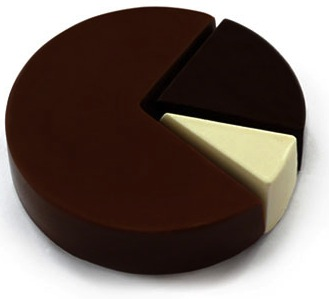
\includegraphics[width=.7in]{pie.jpg} 
   &
   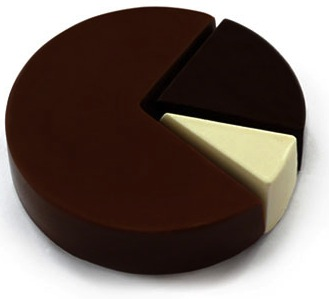
\includegraphics[width=.7in]{pie.jpg} 
   &
   \Huge $\dotsb$
 &
   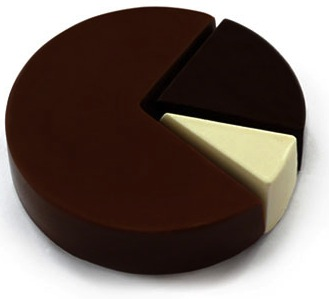
\includegraphics[width=.7in]{pie.jpg} 
\end{tabular}

Have some cheesecake. 
\end{center}


\section{DP Data Mining -- Nice tool to have}
 
For $i = 1, \cdots, n$, 
\begin{eqnarray*}
Y_i &\equiv&  \{X_{i1}, X_{i2}, \cdots, X_{iK}\}\\
Y_i &\sim& \text{Multinomial}(N_i, p_i)\\
 X_{ik} &\in&  \mathbb{N}^+ \cup \{0\}\\
 N_i  &=& \sum_{k=1}^K X_{ik}
\end{eqnarray*}
Model 
\begin{eqnarray*}
p_i &\sim & \text{Dirichlet}(\theta_i)\\ 
\theta_i & \sim & G\\
G &\sim & \text{DP}(\alpha G_0) \\ 
\alpha &\sim& \text{Gamma}(a,b)\\
G_0 &\equiv& \text{Normal}_+(\mu,\Sigma) 
\end{eqnarray*}
Or if that's not quite appropriate for modeling the $p_i$, model, for example, 
\begin{eqnarray*}
p_i & \sim & \text{Dirichlet}(\theta + O_i)\\ 
O_i & \sim & G \\
G & \sim & \text{DP}(\alpha G_0) \\ 
\alpha &\sim& \text{Gamma}(a,b)\\
G_0 &\equiv& \pi \delta_0 + (1-\pi) \text{Normal}(\mu,\Sigma) 
\end{eqnarray*}

Choices for $G_0$ are important.
There's lots of data to do this in an empirical fashion.  
Inference on $\theta$ locates interesting pies $Y_i$ (clusters, perhaps).  
This could be applied across any single hierarchical data level.   
And then I don't have to look through this data for interesting things myself.  

\section{Three level nested data -- DP hierarchical modeling}

For $i = 1, \cdots, n$, 
\begin{eqnarray*}
Y^{(1)}_i &\equiv&  \{X^{(1)}_{i1}, X^{(1)}_{i2}, \cdots, X^{(1)}_{iQ^{(1)}}\}\\
Y^{(1)}_i &\sim& \text{Multinomial}(N_i, p^{(1)}_i)\\
 X^{(1)}_{ij} &\in&  \mathbb{N}^+ \cup \{0\}\\
 N_i  &=& \sum_{j=1}^{Q^{(1)}} X^{(1)}_{ij} \\
 \\
 \\
Y^{(2)}_{ij} &\equiv&  \{X^{(2)}_{ij1}, X^{(2)}_{ij2}, \cdots, X^{(2)}_{ijQ^{(2)}}\}\\
Y^{(2)}_{ij} &\sim& \text{Multinomial}(X^{(1)}_{ij}, p^{(2)}_{ij})\\
 X^{(2)}_{ijk} &\in& \mathbb{N}^+ \cup \{0\}\\
 X^{(1)}_{ij}  &=& \sum_{k=1}^{Q^{(2)}} X^{(2)}_{ijk} \\
 \\
 \\
Y^{(3)}_{ijk} &\equiv&  \{X^{(3)}_{ijk1}, X^{(3)}_{ijk2}, \cdots, X^{(3)}_{ijkQ^{(3)}}\}\\
Y^{(3)}_{ijk} &\sim& \text{Multinomial}(X^{(2)}_{ijk}, p^{(3)}_{ijk})\\
 X^{(3)}_{ijkl} &\in& \mathbb{N}^+ \cup \{0\}\\
 X^{(2)}_{ijk}  &=& \sum_{l=1}^{Q^{(3)}} X^{(3)}_{ijkl} 
\end{eqnarray*}

This is a three level nested data structure:
\begin{itemize}
\item  Individual $i$ has a $1^{st}$ level multinomial random variable, $Y^{(1)}_i$.

\item The $j^{th}$ category in $Y^{(1)}_i$ (with $X^{(1)}_{ij}$ counts) 
may itself be subdivided into a multinomial random variable, $Y^{(2)}_{ij}$. 

\item The $k^{th}$ category in $Y^{(2)}_{ij}$ (with $X^{(2)}_{ijk}$ counts) 
may itself be subdivided into a multinomial random variable, $Y^{(3)}_{ijk}$. 

\item The $l^{th}$ category in $Y^{(3)}_{ijk}$ will have $X^{(2)}_{ijkl}$ counts. 
\end{itemize}

Consider just the top two levels (ignore the bottom third level),
and model 
\begin{eqnarray*} 
p^{(1)}_i &\sim & \text{Dirichlet}(\theta^{(1)} + A_i^{(1)})\\
\theta^{(1)} &\sim& \text{Normal}_+(\mu^{(1)}_{\theta}, \Sigma^{(1)}_{\theta})\\
A_i^{(1)} &\equiv& \{A_{i1}^{(1)}, A_{i2}^{(1)}, \cdots, A^{(1)}_{iQ^{(1)}}\}\\
A_{ij}^{(1)}  &\sim & G_j^{(1)} \\
G_j^{(1)} &\sim& \text{DP}_j(\alpha_j^{(1)} G_{0}^{(1)})\\
\alpha_j^{(1)} &\sim& \text{Gamma}_j(a^{(1)},b^{(1)})\\
G_{0} &\equiv&  \pi^{(1)} \delta_0 + (1-\pi^{(1)})\text{Normal}(\mu_{A}^{(1)}, \sigma_{A}^{(1)}) \\
%\otimes \text{Normal}_+(\mu_{\theta^{(2)}}, \Sigma_{\theta^{(2)}})
\\ 
p^{(2)}_{ij} &\sim & \text{Dirichlet}(\theta^{(2)}_{ij} + A_{ij}^{(2)})\\
\theta^{(2)}_{ij} | A_{ij}^{(1)} = a_{ij} &\sim& 
\text{Normal}_+(\mu^{(2)}_{\theta a_{ij}}, \Sigma^{(2)}_{\theta a_{ij}})\\
A^{(2)}_{ij} &\equiv& \{A^{(2)}_{ij1}, A^{(2)}_{ij2}, \cdots, A^{(2)}_{ijQ^{(2)} }\}\\
A^{(2)}_{ijk} | A_{ij}^{(1)} = a_{ij} &\sim & G_{jk a_{ij}}^{(2)}\\ 
G_{jk a_{ij}}^{(2)} &\sim & \text{DP}_{jk a_{ij}}(\alpha_{jk a_{ij}}^{(2)} G^{(2)}_{0})\\
\alpha_{jk a_{ij}}^{(2)} &\sim& \text{Gamma}_{jk a_{ij}}(a^{(2)},b^{(2)})\\
G_{0} &\equiv& \text{Normal}(\mu^{(2)}_{A}, \sigma^{(2)}_{A}) 
\end{eqnarray*}

\begin{itemize}
\item The DPs cluster the $i$'s element wise on the $A$ adjustments.
\item Each of the elements  in the $A$ adjustment become a new multinomial
random variable.   The clusters get the same $\theta^{(2)}$. 
\item The extension from the second to the third level would be 
analogous to that of the extension from the first to the second. 
\item I view this as some kind of bubbling process.  
When there's a cluster in a top level category, those in the 
cluster grow a separate parameter in the next level.
\item Writing this out is all well and good... fitting this thing is going to be something else.
\item I also am not sure if a difference between a category at one level 
means that there should be a difference in the next level breakdown of that 
category... but that's what we're doing here.    
\end{itemize}


\end{document}  

Model 
\begin{eqnarray*} 
p^{(1)}_i &\sim & \text{Dirichlet}(\theta_i)\\ 
p^{(2)}_{ij} \\ 
\theta_i & \sim & \text{DP}(\alpha G_0) \\ 
\alpha &\sim& \text{Gamma}(a,b)\\
G_0 &\equiv& \text{Normal}_+(\mu,\Sigma) 
\end{eqnarray*}

